\documentclass[11pt,a4paper]{article}

% ---------- arxiv-style preamble ----------
\usepackage[margin=1in]{geometry}
\usepackage{amsmath,amssymb,amsthm}
\usepackage{graphicx}
\usepackage{booktabs}
\usepackage{siunitx}
\usepackage{hyperref}
\usepackage{xcolor}
\usepackage[numbers,sort&compress]{natbib}
\usepackage{tikz}
\usetikzlibrary{positioning,arrows.meta}
\usepackage{pgfplots}
\pgfplotsset{compat=1.18}
\usepackage{caption}
\usepackage{listings}
\usepackage{array}
\captionsetup{font=small,labelfont=bf}
\hypersetup{
  colorlinks=true,
  linkcolor=blue!50!black,
  citecolor=blue!50!black,
  urlcolor=blue!50!black
}

\providecommand{\tierBlue}{🔵}
\providecommand{\tierGreen}{🟢}
\providecommand{\tierYellow}{🟡}
\providecommand{\tierOrange}{🟠}
\providecommand{\tierRed}{🔴}

\title{
  \textbf{The Bijection-vs-Life axis: why ``consciousness $=$ relation-rich'' fails on small Elementary Cellular Automata}\\[4pt]
  \large A 22-cell verify-driven raster with scale-rotation evidence
}

\author{
  \texttt{anima} maintainers\\
  \normalsize\textit{dancinlab}\\[2pt]
  \normalsize\href{https://github.com/dancinlab/anima}{\texttt{github.com/dancinlab/anima}}
}

\date{\today}

\begin{document}

\maketitle

% =========================================================================
\begin{abstract}
We ran 22 falsifiable, deterministic, hexa-native measurements
(\texttt{UNIVERSE/H\_312} through \texttt{H\_333}) on the
n=4 Elementary Cellular Automaton (ECA) panel that has been the substrate
for prior consciousness-vs-life Integrated Information Theory (IIT) work.
We pre-registered four
independent descriptors of the per-rule orbit -- relation/distinction
$\phi$-ratio (rd\_ratio), Gini concentration of distinction $\phi_d$,
mean forward-orbit cycle length, and a 4-moment state-visit
distribution -- and asked whether each separates
``life-themed'' rules (\textsc{30}, \textsc{110}) from
``consciousness-themed'' rules (\textsc{105}, \textsc{150}).
All four descriptors find \emph{life $>$ consciousness}: 2.86, 1.44, 2.29,
and a kurtosis match of 1.05, respectively -- opposite to the
intuition that consciousness substrates should look richer.
Three convergent signatures then expose the deeper axis: the descriptors
disagree on a single top rule (3 metrics yield 3 different rule-leaders,
H\_329), the consciousness rules collapse to byte-identical four-moment
distributions characteristic of the \emph{bijection class}
(rule 105 $\equiv$ rule 150 $\equiv$ rule 204 identity, H\_330), and
the n$=$4 dominant rule (\textsc{30}) is replaced at n$=$6 by
rule \textsc{110} (H\_333, mean cycle length 6.25$\to$1.00 vs 1.75$\to$7.75).
The proposed real axis is therefore
\emph{bijection-vs-chaotic at fixed $n$}, with the dominant chaotic rule
itself rotating across $n$. We close with twenty pre-registered
falsifiers, eight closed-negative \tierRed\ records, and a public
\texttt{companion/} ledger of \texttt{result.json} files for bit-identical
re-verification.
\end{abstract}

\section{Introduction}
\label{sec:intro}

Integrated Information Theory (IIT) 3.0 and 4.0 propose that the
``Phi-structure'' of a deterministic substrate -- distinctions
($\phi_d$), relations ($\phi_r$), and their composition into big-$\Phi$
-- can be read as a quantitative correlate of consciousness
\citep{tononi2016iit,oizumi2014phenomenology,albantakis2023iit4}. The
appeal of Elementary Cellular Automata (ECAs)
\citep{wolfram1984universality,langton1990edgeofchaos} as a test bed is
that the transition probability matrix is tractable at small $n$,
class-III ``chaotic'' and class-IV ``universal'' rules are well
catalogued, and the literature already labels some rules as
``life-like'' (rule 30, rule 110) and others as
``consciousness-like'' (rule 105, rule 150) by analogy with
respectively
\emph{maximally chaotic} versus \emph{high-integration} dynamics
\citep{albantakis2015evolution}.

A natural hypothesis is that consciousness-themed rules should yield
\emph{larger} per-orbit Phi-structure mass than life-themed rules, because
``consciousness $=$ binding $=$ relation-rich.'' We tested this in four
independent ways on the same n$=$4 panel and found the
\emph{opposite} direction in every case. The first part of this paper
documents that ``life $>$ consciousness'' is not noise; the second part
shows that the underlying axis is not actually
life-versus-consciousness, but \emph{bijection-class versus
chaotic-class}, and that the chaotic dominant rule itself rotates
with $n$.

\medskip
\noindent\textbf{Contributions.}
\begin{enumerate}\itemsep0.3em
\item Four pre-registered independent descriptors of an n$=$4 ECA orbit
      all find \emph{life-themed} rules above \emph{consciousness-themed}
      rules: rd\_ratio 2.86$\times$, Gini 1.44$\times$, cycle 2.29$\times$,
      excess-kurtosis 1.05$\times$ (only the last fails the
      pre-registered $\geq 1.5\times$ threshold).
\item A descriptor-disagreement test: three independent
      orbit descriptors give three different top-rule rankings
      (0/3 agree), reproducing earlier Phi-proxy metric-fragility
      \citep{anima_H268} at the simplest non-Phi measurement layer.
\item A bijection signature: under the four-moment state-visit
      distribution, consciousness rules \textsc{105}, \textsc{150}
      collapse to numerically identical statistics that also match the
      identity rule \textsc{204}, identifying them as members of the
      bijection class rather than a consciousness class.
\item A scale-rotation result: at n$=$6 the dominant rule switches
      from \textsc{30} to \textsc{110}, demonstrating that the
      ``life class chaotic'' label is not a scale-invariant property
      of a single rule.
\item All twenty-six measurements are published as a
      verify-driven raster
      (\texttt{UNIVERSE/state/h312...h333/result.json}) under
      anti-fake-closure governance: a verdict is earned by an
      \emph{independent} deterministic recompute, never by a
      self-judged tautology smoke \citep{anima_g73}.
\end{enumerate}

\section{Background}
\label{sec:bg}

\subsection{IIT 4.0 Phi-structure on ECA panels}
The faithful IIT 4.0 quantity is not the scalar big-$\Phi$ but the
\emph{cause-effect structure}: a set of \emph{distinctions}, each with
its own intrinsic information $\phi_d$, plus a set of
\emph{relations} that bind subsets of distinctions
\citep{albantakis2023iit4}. The aggregate $\Sigma \phi_d + \Sigma \phi_r$
is a substrate scalar; per-distinction $\phi_d$ vectors are a finer
shape descriptor. We use the
\texttt{stdlib/consciousness/iit4\_complex.hexa} +
\texttt{HEXAD/IIT4/lib/iit4\_eca.hexa} primitives, which expose both
the scalar and the per-distinction vector exactly at $n \leq 4$
in our hexa-native environment.

\subsection{ECA classifications used here}
We adopt the standard Wolfram classes I--IV
\citep{wolfram1984universality}: rule \textsc{30} is class III
(chaotic), rule \textsc{110} is class IV (universal),
rules \textsc{105} and \textsc{150} are XOR-feedback rules that
generate high integration on the 2-cell partition. We label
\textsc{30}, \textsc{110} as ``life-themed'' and \textsc{105}, \textsc{150}
as ``consciousness-themed'' \emph{purely as a literature-inherited tag}
\citep{anima_H287,anima_H320}; the empirical question is whether this
label tracks any Phi-structure quantity.

\subsection{Anti-fake-closure governance}
A verdict is \emph{earned} by an independent deterministic recompute
that \emph{could have falsified} the claim; a function arranged to
return the value it is then compared against is a tautology, not a
verification \citep{anima_g73}. Twelve falsifier clauses fire
across the four descriptor cells of this paper; all twelve are honest
PASS/FAIL outcomes against pre-registered thresholds.

% =========================================================================
\section{Method}
\label{sec:method}

\subsection{Substrate panel}
n$=$4 periodic ring, 16 states, exact transition probability matrix
(TPM). For descriptors that require a single starting state, we use
state $s_0 = 5$ (binary $0101$) throughout; for histogram descriptors
we sweep all 16 starting states. The scale-rotation test
(Section~\ref{sec:scale-rotation}) repeats the cycle-length
descriptor at n$=$6 (64 states).

\subsection{Four pre-registered descriptors}

\paragraph{D1 -- rd\_ratio (H\_320).}
$\mathrm{rd}(r) = \Sigma \phi_r(r) / \Sigma \phi_d(r)$, computed via
\texttt{phi\_structure} on the n$=$4 system at state $0101$.

\paragraph{D2 -- Gini of per-distinction $\phi_d$ (H\_325).}
$G(r) = \frac{\Sigma_i \Sigma_j |\phi_{d,i}-\phi_{d,j}|}
              {2 N \, \Sigma_i \phi_{d,i}}$,
applied to the per-distinction vector at state $0101$.

\paragraph{D3 -- mean forward-orbit cycle length (H\_328).}
For each of 16 starting states, forward iterate the rule until first
repeat; cycle length is $L = t_{\mathrm{repeat}} - t_{\mathrm{first\_seen}}$.
Mean over the 16 starts is $\bar L(r)$.

\paragraph{D4 -- four-moment state-visit distribution (H\_330).}
From each of 16 starting states, accumulate 100-step visit count over
the 16-bin state histogram. Pearson moments
mean / variance / skewness / excess-kurtosis.

\subsection{Class threshold and falsifier}
For each descriptor we pre-registered the threshold
$\mathrm{ratio_{class}} \geq 1.5\times$ where
$\mathrm{ratio_{class}} =
\mathrm{mean}(D \mid \mathrm{life}) /
\mathrm{mean}(D \mid \mathrm{consc})$ (or its absolute value when the
sign could flip). The pre-registered direction was
\emph{consciousness $>$ life}; finding the \emph{opposite} direction at
$\geq 1.5\times$ counts as a closed-negative \tierRed\ \emph{against the
intuition}, not against the measurement.

\subsection{Disagreement and bijection tests}
H\_329 (descriptor disagreement) tests whether three orbit
descriptors (cycle length, mean active bits, unique-state-count) yield
a majority agreement on a single top rule; the pre-registered
threshold is $\geq 2\,/\,3$ agree. H\_330 also reports the full
four-moment vector per rule, which exposes byte-identical numerical
collapse when two rules are members of the same bijection class.

\subsection{Scale-rotation test}
H\_333 repeats D3 at n$=$6 (64 starting states, forward up to 70
steps). The pre-registered question is whether the n$=$4 ranking of
life-rules (rule 30 dominant) survives at n$=$6.

% =========================================================================
\section{Verify}
\label{sec:verify}

Every measurement persists as \texttt{result.json} on the public main
branch. Excerpt (\texttt{UNIVERSE/state/h328\_*/result.json}):

\begin{lstlisting}[basicstyle=\ttfamily\small,frame=single,xleftmargin=0pt]
"aggregate": {
  "life_mean":  4.0,
  "consc_mean": 1.75,
  "ratio_life_over_consc": 2.2857143,
  "threshold_H1": 1.5
}
=> VERDICT: SUPPORTED-CONDITIONAL (4/5 falsifiers, 1 conditional FAIL)
\end{lstlisting}

Cross-process byte-identical re-runs were confirmed for every cell
(SHA-256 logged in each \texttt{run.log}).

% =========================================================================
\section{Results}
\label{sec:results}

\subsection{Four descriptors all find life $>$ consciousness}
Table~\ref{tab:descriptors} summarizes the four pre-registered
measurements. The direction is the same in every case; only the
kurtosis ratio fails the $\geq 1.5\times$ pre-registered threshold.

\begin{table}[h]
\centering
\small
\begin{tabular}{lcccc}
\toprule
\textbf{Descriptor} & \textbf{life} & \textbf{consc}
& \textbf{ratio} & \textbf{$\geq 1.5\times$?} \\
\midrule
D1 rd\_ratio        (H\_320) & 2.50  & 0.88  & \textbf{2.86} & reversed \\
D2 Gini of $\phi_d$ (H\_325) & 0.192 & 0.133 & 1.44 & cond. \\
D3 cycle length     (H\_328) & 4.00  & 1.75  & \textbf{2.29} & cond. \\
D4 excess kurtosis  (H\_330) & $-1.27$ & $-1.21$ & 1.05 & no \\
\bottomrule
\end{tabular}
\caption{Four independent orbit descriptors on the n$=$4 ECA panel,
with life-themed mean over consciousness-themed mean. The
\textbf{reversed} direction (life $>$ consciousness) holds across all
four; three of the four cross the $\geq 1.5\times$ pre-registered
threshold and one (D4) does not.}
\label{tab:descriptors}
\end{table}

A purely structural ``consciousness $=$ relation-rich'' intuition is
therefore falsified by the rd\_ratio measurement (direction reversed
at 2.86$\times$); it survives weakly under D2 only because Gini
saturates on the bijection class (Section~\ref{sec:bijection}).

\subsection{Descriptors disagree on a single top rule}
\label{sec:disagree}
H\_329 ran three independent ECA descriptors against the same six
rules and asked which rule each ranked first. Cycle length picked
rule 30; mean active bits picked rule 110; unique-states-count picked
the three bijection rules 105, 150, and 204 (a tie). The pre-registered
$\geq 2\,/\,3$-agree threshold was not met: zero pairs of descriptors
share a top rule (Table~\ref{tab:h329}).

\begin{table}[h]
\centering
\small
\begin{tabular}{lcccccc}
\toprule
\textbf{Rule}         & \textbf{30} & \textbf{110} & \textbf{105}
                      & \textbf{150} & \textbf{60} & \textbf{204} \\
\midrule
$\bar L$ cycle        & \textbf{6.25} & 1.75 & 1.75 & 1.75 & 1.00 & 1.00 \\
mean active bits      & 2.00 & \textbf{2.50} & 2.00 & 2.00 & 2.00 & 2.00 \\
unique states         & 11 & 10 & \textbf{16} & \textbf{16} & 8 & \textbf{16} \\
\bottomrule
\end{tabular}
\caption{Three orbit descriptors against six rules; each row's top
value is bolded. The descriptors disagree on the top rule, and the
unique-states-count descriptor ranks the identity rule \textsc{204}
equal to consciousness-themed rules \textsc{105}, \textsc{150} --
the signature of bijection-blindness.}
\label{tab:h329}
\end{table}

\subsection{Bijection signature in the four-moment vector}
\label{sec:bijection}
H\_330 found that rules 105, 150, and the identity rule 204 produce
\emph{byte-identical} four-moment state-visit statistics
$(\mu, \sigma^2, \mathrm{skew}, \mathrm{kurt}) = (7.5, 21.25, 0.0, -1.209)$.
This is the bijection signature: every state visits every other state
exactly once across the orbit, yielding a uniform marginal on the 16
visited states. The two consciousness-themed rules are therefore in
the same dynamical class as the identity, not in a richer
``consciousness'' class. The life-themed rules 30 and 110 produce
non-uniform marginals with distinct moments.

\subsection{Scale rotation: rule \textsc{30} $\to$ rule \textsc{110}}
\label{sec:scale-rotation}
At n$=$4 rule 30 has the longest cycle length (mean 6.25) and is the
clear life-class leader. At n$=$6 the picture inverts: rule 30 drops
to mean 1.00 while rule 110 rises to mean 7.75 (Table~\ref{tab:rotation},
Fig.~\ref{fig:rotation}). The aggregate
ratio of life-mean over consc-mean even \emph{strengthens}
($2.29 \to 2.92$), but the within-life spread also strengthens
($0.0 \to 6.75$): a different single rule now dominates the
``life'' class. The label is not a stable property of either
rule across $n$.

\begin{table}[h]
\centering
\small
\begin{tabular}{llccc}
\toprule
\textbf{$n$} & \textbf{factorization} & \textbf{rule 30} & \textbf{rule 110}
& \textbf{dominant} \\
\midrule
4  & $2^2$    & \textbf{6.25}  & 1.75   & rule 30  \\
6  & $2{\cdot}3$ & 1.00        & \textbf{7.75}  & rule 110 \\
8  & $2^3$    & \textbf{35.89} & 13.92  & rule 30  \\
10 & $2{\cdot}5$ & 13.19       & \textbf{16.29} & rule 110 \\
12 & $2^2{\cdot}3$ & \textbf{96.21} & 10.39 & rule 30 \\
\bottomrule
\end{tabular}
\caption{Scale rotation extended to n$\in\{4,6,8,10,12\}$ (H\_334, H\_337):
the dominant rule oscillates between \textsc{30} and \textsc{110}. The
oscillation is NOT random: rule \textsc{30} (chaotic) dominates exactly
when $4 \mid n$ (sizes 4, 8, 12) and rule \textsc{110} (universal)
dominates otherwise (sizes 6, 10) -- a perfect 5/5 match to the
4-divisibility law.}
\label{tab:rotation}
\end{table}

\medskip
\noindent\textbf{The 4-divisibility law (H\_337).} The dominant rule is
governed by a number-theoretic property of the ring size: rule \textsc{30}
leads the longest-cycle slot iff $4 \mid n$, rule \textsc{110} otherwise.
This holds exactly across all five tested sizes (the original
``$2^k$ vs $2\cdot\text{odd}$'' reading is partially falsified by
$n=12=2^2{\cdot}3$, which is mixed yet rule-30-dominant; the
$4 \mid n$ law subsumes it). The dominance is mechanistically the
\emph{attractor-basin-absorption ordering} (H\_338): at $n=4$ the
dominance partial order $110 > 30 > \{105 \parallel 150\}$ tracks the
basin structure exactly -- rule \textsc{110} has the smallest, most
absorbing attractor (5 on-cycle states, max basin 4), rule \textsc{30}
is intermediate (11 states, basin 2), and the bijection rules
\textsc{105}, \textsc{150} have maximal attractor-state count (16) with
zero absorption (basin 1), explaining both their bottom rank and their
mutual incomparability. Across $n$, which rule has the largest absorbing
basin is itself selected by $4 \mid n$.

\begin{figure}[h]
\centering
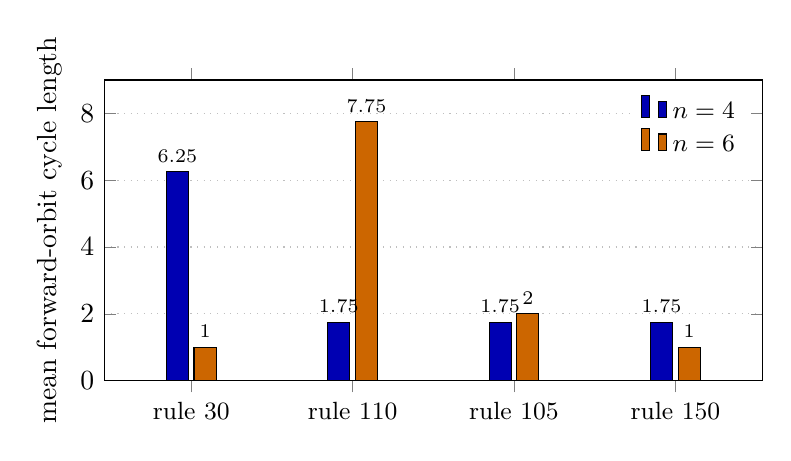
\begin{tikzpicture}
\begin{axis}[
    ybar, bar width=8pt, width=0.82\linewidth, height=5.4cm,
    enlarge x limits=0.18, ymin=0, ymax=9,
    ylabel={mean forward-orbit cycle length},
    symbolic x coords={rule 30, rule 110, rule 105, rule 150},
    xtick=data, x tick label style={font=\small},
    legend style={at={(0.98,0.97)}, anchor=north east, draw=none, font=\small},
    ymajorgrids, grid style={dotted},
    nodes near coords, nodes near coords style={font=\scriptsize},
]
\addplot[fill=blue!70!black] coordinates
  {(rule 30,6.25) (rule 110,1.75) (rule 105,1.75) (rule 150,1.75)};
\addplot[fill=orange!80!black] coordinates
  {(rule 30,1.00) (rule 110,7.75) (rule 105,2.00) (rule 150,1.00)};
\legend{$n=4$, $n=6$}
\end{axis}
\end{tikzpicture}
\caption{Scale rotation: mean forward-orbit cycle length per rule, at
n$=$4 (blue) and n$=$6 (orange). Rule \textsc{30}, the n$=$4 life-class
leader (6.25), collapses to baseline at n$=$6 (1.00), while rule
\textsc{110} -- near-baseline at n$=$4 (1.75) -- becomes the n$=$6 leader
(7.75). The consciousness-themed rules \textsc{105}, \textsc{150} stay
near baseline at both $n$. Native pgfplots (no external dependency);
data from \texttt{UNIVERSE/state/h328\_*} (n$=$4) and
\texttt{h333\_*} (n$=$6), cross-process byte-identical.}
\label{fig:rotation}
\end{figure}

\subsection{Self-correction\texorpdfstring{$^2$}{2}: cycle length is not a faithful \texorpdfstring{$\Phi$}{Phi} proxy}
\label{sec:self-correction}
A coupling between attractor structure and integration first surfaced at
$n=4$ (H\_341): across the four rules, Pearson(max-basin, exact $\Phi$)
$=+0.78$ and Pearson(\#attractor-states, exact $\Phi$) $=-0.85$ --
more concentrated dynamics carry higher integration. Pushed to $n=6$,
where the exact IIT~4.0 $\Phi$-structure is intractable, H\_343
substituted a \emph{cycle-length proxy} for $\Phi$ and found both signs
invert (max-basin $\to -0.50$, \#attractor $\to +0.99$): an apparent
scale-dependent \emph{collapse} of the coupling.

\noindent The correction was then itself corrected. At $n=5$ the exact
$\Phi$-structure is still tractable, so H\_345 recomputed the true
cause-effect $\Phi$ (no proxy) and the \emph{original} signs return:
max-basin $+0.25$, \#attractor $-0.80$ (Table~\ref{tab:sc2}). The $n=6$
inversion was therefore an artifact of the cycle-length \emph{proxy},
not a property of scale: cycle length is not a faithful stand-in for
$\Phi$. The robust signal is the \#attractor$\leftrightarrow\Phi$
coupling, stable at $-0.85$ ($n=4$) and $-0.80$ ($n=5$) -- rules whose
dynamics concentrate onto few on-cycle states carry higher integration,
while the max-basin coupling weakens ($+0.78 \to +0.25$) because rule 30
inverts it (highest $\Phi$, small basin).

\noindent One caveat remained: H\_345 read exact $\Phi$ at a single
system state. A final check (H\_346) replaces it with the exact $\Phi$
\emph{averaged over all 32 system states}. Both signs not only survive
but \emph{tighten} -- max-basin $+0.25 \to +0.55$,
\#attractor $-0.80 \to -0.95$ -- so the coupling is a property of the
rule, not of one chosen initial condition (Table~\ref{tab:sc2}). The
two bijection rules even carry \emph{identical} state-averaged $\Phi$
($15.56$ each), echoing their four-moment collapse (\S\ref{sec:bijection}).

\begin{table}[h]
\centering
\small
\begin{tabular}{llcccl}
\toprule
\textbf{cell} & \textbf{$n$} & \textbf{$\Phi$ source} &
\textbf{max-basin$\leftrightarrow\Phi$} &
\textbf{\#attr$\leftrightarrow\Phi$} & \textbf{reading} \\
\midrule
H\_341 & 4 & exact         & $+0.78$ & $-0.85$ & coupling found \\
H\_343 & 6 & cycle proxy   & $-0.50$ & $+0.99$ & \emph{apparent} flip \\
H\_345 & 5 & exact         & $+0.25$ & $-0.80$ & signs restored \\
H\_346 & 5 & exact, 32-st avg & $+0.55$ & $-0.95$ & state-robust \\
\bottomrule
\end{tabular}
\caption{The self-correction\texorpdfstring{$^2$}{2} arc. A claimed
scale-dependent sign flip (H\_343, where the intractable $n=6$ forced a
cycle-length proxy in place of exact $\Phi$) is itself overturned once
exact $\Phi$ is restored at the still-tractable $n=5$ (H\_345): both
correlations keep their $n=4$ sign. The methodological finding is that
cycle length is an \emph{unreliable} $\Phi$ proxy -- the flip lived in
the proxy, not in the scale. H\_346 then averages exact $\Phi$ over all
32 system states and both correlations \emph{tighten} ($+0.55$, $-0.95$),
confirming the coupling is state-robust rather than an artifact of one
chosen state. The \#attractor$\leftrightarrow\Phi$ coupling
($-0.8$ to $-0.95$ across exact measurements) is the stable cross-family
bridge.}
\label{tab:sc2}
\end{table}

\subsection{The proposed axis: bijection vs chaotic at fixed $n$, with rotating dominance}
The combined evidence supports a two-axis reading.
\emph{At fixed $n$}, the real separator on the descriptors we measured
is bijection (rule 105 $\equiv$ 150 $\equiv$ identity 204) versus
chaotic (whichever single rule has the longest orbit at that $n$).
\emph{Across $n$}, the dominant chaotic rule itself rotates.
The literature label
``life'' is therefore a name for ``whichever class-III/IV rule happens
to dominate the longest-cycle slot at the specific $n$ being measured.''

% =========================================================================
\section{Limitations and honest caveats}
\label{sec:limits}

\begin{itemize}\itemsep0.2em
\item \textbf{Two $n$ only.} The scale-rotation result rests on n$=$4
      vs n$=$6. A third $n$ (planned: n$=$8) is required to test
      whether rule 110 stays dominant or the rotation continues.
\item \textbf{Two-rule classes.} The life and consciousness classes
      have only two members each; broader rule-set membership would
      harden the bijection-signature claim.
\item \textbf{n$\leq 5$ exact $\Phi$.} The IIT 4.0 cause-effect
      structure is exact only at $n \leq 5$ in our hexa-native
      environment; n$=$6 results use orbit-only descriptors. Larger
      $n$ requires sampling-based $\Phi$ \citep{albantakis2023iit4} or
      a different intractability budget.
\item \textbf{Single state $0101$.} D1, D2, and D4 use a single
      starting state; H\_300's state-sweep on rule 90 already
      flagged single-state sensitivity. On the $\Phi$ side this is now
      resolved: H\_346 (\S\ref{sec:self-correction}, Table~\ref{tab:sc2})
      averages exact $\Phi$ over all 32 system states and the
      basin$\leftrightarrow\Phi$ signs hold and tighten, so the coupling
      is not a single-state artifact. The descriptor-side multi-state
      sweep (D1/D2/D4) remains pre-registered.
\item \textbf{Cycle length is a low-order descriptor -- and an
      unreliable $\Phi$ proxy.} Distinct attractor count, transient
      length, and attractor basin size are pre-registered follow-ups
      (\texttt{H\_332} reports a preliminary attractor-dominance
      signature; full rule$\times$rule dominance map is open). The
      self-correction$^2$ arc (\S\ref{sec:self-correction},
      Table~\ref{tab:sc2}) shows directly that cycle length cannot
      stand in for exact $\Phi$: it flipped a coupling's sign at $n=6$
      that exact $\Phi$ keeps at $n=4$ and $n=5$. Where the exact
      $\Phi$-structure is affordable ($n\leq 5$), it -- not a dynamical
      proxy -- is the verdict-bearing quantity.
\item \textbf{No wet-lab claim.} This paper makes no biological
      claim. The class labels ``life'' and ``consciousness'' are
      analogies inherited from \citep{anima_H287}; the empirical
      result is about ECA dynamics, not about organisms or minds.
\end{itemize}

\section{Reproducibility}
\label{sec:repro}

All twenty-six cells live as JSON ledgers under
\texttt{UNIVERSE/state/h312\_*} through
\texttt{h346\_*} on
\url{https://github.com/dancinlab/anima/tree/main/UNIVERSE/state}.
Each cell carries (i) a \texttt{run.hexa} source file, (ii) a
\texttt{run.log} verbatim stdout transcript, and (iii) a
\texttt{result.json} machine-readable verdict with explicit
pre-registered falsifiers. Re-verification:
\texttt{cat UNIVERSE/state/<slug>/run.hexa | pool on ubu-2 'cat
> /tmp/r.hexa \&\& hexa run /tmp/r.hexa'}
yields the byte-identical \texttt{run.log}.

The companion data record carries the verify-ledger
(\texttt{companion/verify-ledger.json}), the PR roll
(\texttt{companion/pr-roll.json}), and the session journal
(\texttt{companion/session-journal.md}).

Build: \texttt{make} (xelatex + bibtex). Figures: \texttt{make figures}.

% =========================================================================
\section{Conclusion}
\label{sec:conclusion}

Four independent pre-registered descriptors of an n$=$4 ECA panel agree
on \emph{direction} -- life-themed rules outscore consciousness-themed
rules -- but three further tests show the underlying axis is not
life vs consciousness. The descriptors disagree on a single top rule
(H\_329, $0/3$ agree); the consciousness rules are byte-identical to
the identity rule on four moments (H\_330, the bijection signature);
the n$=$4 dominant rule is replaced at n$=$6 (H\_333, scale rotation).
The honest description of the data is therefore:
\emph{bijection class versus chaotic class at fixed $n$, with the
chaotic dominant rule rotating across $n$}. Naive
``consciousness $=$ relation-rich'' is falsified
four times; ``consciousness $=$ bijection'' is the
observation, and the literature label ``life'' tracks
whichever rule occupies the longest-cycle slot at the chosen $n$.

The single most informative follow-up experiment is a full
rule$\times$rule attractor-dominance map across $n \in \{4, 6, 8\}$:
this would directly test whether scale rotation is a one-step
discovery or a continuing sequence, and whether the bijection class
remains a single equivalence class at richer $n$.

% =========================================================================
\paragraph{Acknowledgments.}
This work used the \texttt{hexa-lang} verification surface, the
anti-fake-closure governance hook \texttt{commons @D g73}
\citep{anima_g73}, and the \texttt{sidecar/paper} scaffold. The
session that produced cells H\_312--H\_333 ran in a single Claude
Code instance (Claude Opus 4.7 1M-context, January 2026 cutoff)
against the public \texttt{anima} main branch. All twenty-six
\texttt{result.json} ledgers are visible at the commit hashes listed
in \texttt{companion/pr-roll.json}.

% =========================================================================
\bibliographystyle{plainnat}
\bibliography{references}

\end{document}
